%\begin{figure}[h]
%\centering
%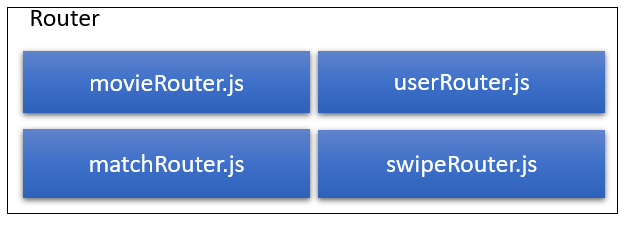
\includegraphics[width=8cm]{images/routestruktur.PNG}
%\caption{Node.js Server - Controller Struktur}
%\end{figure}
In der Server.js werden dem Express-Objekt 'app' die einzelnen Routen für die Weiterleitung der HTTPS-Anfragen an die entsprechenden Controller hinzugefügt. Dabei werden die zu den Anfragen gehörenden Request- und Response-Objekte als Parameter an die Controller übergeben.

\begin{lstlisting}[caption=Routing in server.js, label=lst:routingserver]
//Movies
const moviesRouter = require('./routes/movies')
app.use('/movies', moviesRouter)

//Users
const usersRouter = require('./routes/users')
app.use('/users', usersRouter)

//Matches
const matchesRouter = require('./routes/matches')
app.use('/matches', matchesRouter)

//Swipes
const swipesRouter = require('./routes/swipes')
app.use('/swipes', swipesRouter)

\end{lstlisting}

\paragraph{Movie Router}
Innerhalb des Movie Routers wird die '/movies/request' an die Funktion RequestMovie des Movie-Controller weitergeleitet.
\begin{lstlisting}[caption=Routing in movieRouter.js, label=lst:routingmovie]
// Require controller modules.
const MovieController = require('../controllers/movieController')

// Send Requests to MovieController
router.post('/request', MovieController.RequestMovies)
\end{lstlisting}

\paragraph{User Router}
Der User Router leitet '/users/create', '/users/change' und '/users/info' an die entsprechenden Funktionen des User-Controllers weiter.
\begin{lstlisting}[caption=Routing in userRouter.js, label=lst:routinguser]
// Require controller modules.
const UserController = require('../controllers/userController')

// Send Request to UserController
router.post('/create', UserController.CreateUser)
router.post('/change', UserController.ChangeUser)
router.post('/info', UserController.InfoUser)
\end{lstlisting}

\paragraph{Match Router}
Innerhalb des Match Routers werden die unten dargestellten URL's an die Funktion des Match-Controller weitergeleitet.

\begin{lstlisting}[caption=Routing in matchRouter.js, label=lst:routingmatch]
// Require controller modules.
const MatchController = require('../controllers/matchController')

// Send Request to MatchController
router.post('/request', MatchController.RequestMatches)
router.post('/deleteSupermatch',MatchController.DeleteSupermatch)
router.post('/deleteNormalmatch',MatchController.DeleteNormalmatch)
router.post('/received', MatchController.Received)
router.post('/trigger', MatchController.Trigger)
\end{lstlisting}


\paragraph{Swipe Router}
Der Swipe Router leitet '/swipes/create' an die entsprechende Funktionen des Swipe-Controllers weiter.

\begin{lstlisting}[caption=Routing in swipeRouter.js, label=lst:routingswipe]
// Require controller modules.
const SwipeController = require('../controllers/swipeController')

// Send Request to SwipeController
router.post('/create',  SwipeController.CreateSwipe )
\end{lstlisting}








